\chapter{Experimental Setup}
Every theory needs experimental proof. Particle physics is tested on colliders.
\\
\\
The Standard Model was experimentaly tested up to scale of ~TeV, Needed to go higher to 
study electroweak symmetry breaking and Higgs mechanism.
\\
\\
Physics beyond SM is also of interest on the scales $>$1TeV.
\\
\\
Previous colliders - designed up to 1 TeV. LHC \cite{LHCmachine} was working with the energy
up to 8 TeV - eightfold increase of energy, many physics perspectives.
\\
\\
One of the general purpose detectors on the LHC is CMS.
\\
\\
This chapter - 2 parts. About LHC and CMS
\\
\\

\section{Large Hadron Collider}

The fastest protons in the world, ever controlled by human , are live in Switzerland at CERN.
The Machine which can manage the operation of these protons is called Large Hadron Collider(LHC). 
The LHC is a ring-shape tunnel 26.7 km long  placed 45 -170 meter ungrounded. 
Inside the tunnel there are two rings with vacuum tubes where proton beams are circulating in different directions.
There are four locations where tings are crossing and the protons can collide with each other. 
The designed center-of-mass energy for those collisions is $\sqrt{s}$ = 14 TeV, which means 7 TeV in one direction.


To not get out of the ring 7 TeV protons are guiding by supperconducting magnets. 



[http://www.lhc-closer.es/1/3/10/0]

To kep running LHC during the 2012 data taking periud was used only 1 cubic suntemiter of H2 gass.

The LHC is the largest experimental facility ever built, at European Organization for Nuclear research, CERN.
\\
\\
LHC - two ring superconductiong proton-proton (or lead nuclei) collider. 
\\
\\
The circumference of the ring is 26.7 km which was former used for the LEP experiment.
\\
\\
It lays under the surfaces of Switzerland and France on the depth 50 to 170 m.
\\
\\
------Designed center-of-mass energy for proton beams -- 14 TeV. It is reached in several steps in preaccelerator system of LHC
and afterwards injected to the largest ring.
\\
\\
The whole accelerator system is on Fig.\ref{fig:AccelCERN}.
\begin{figure}[t]
  \centering
  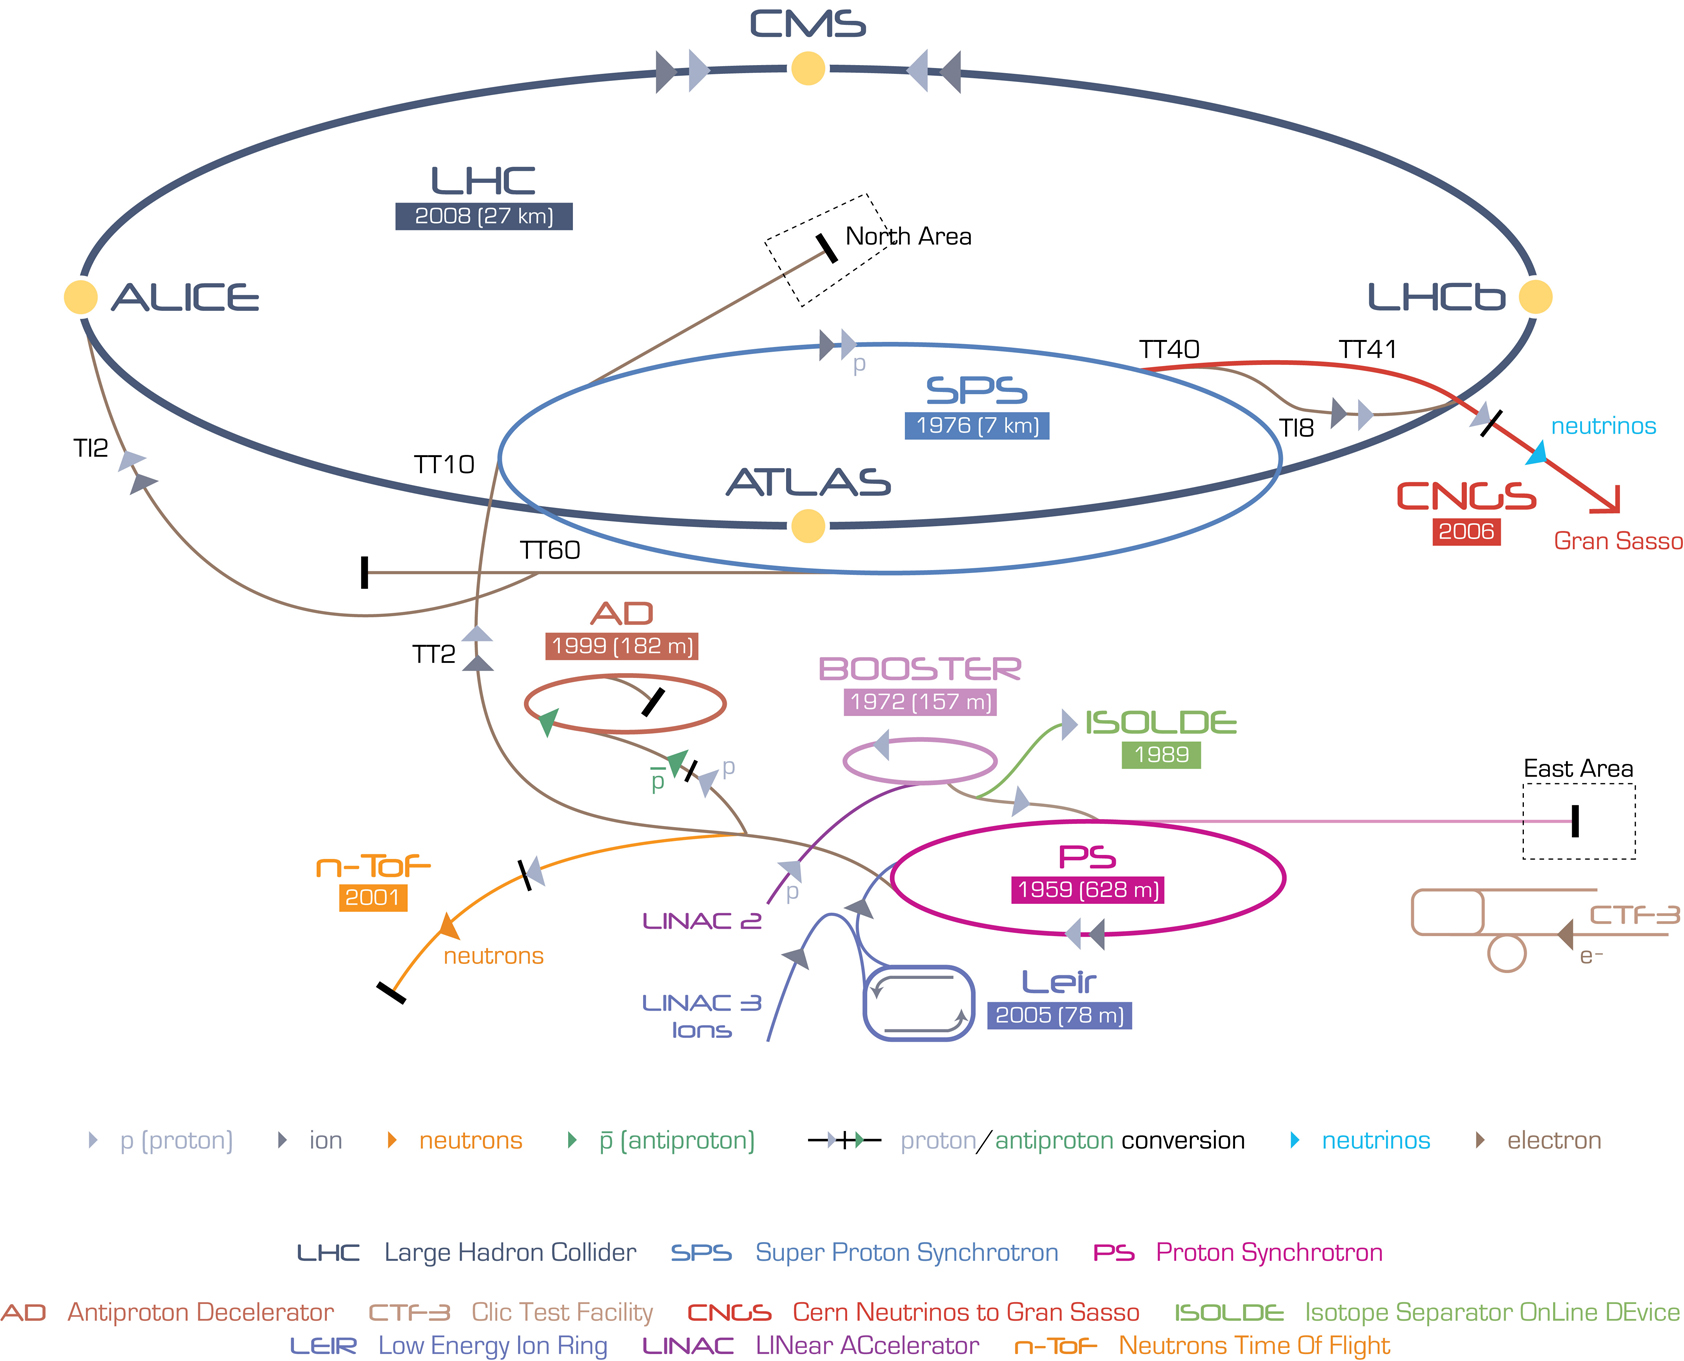
\includegraphics[width=0.6\textwidth]{02_experimental_setup/plots/Cern-Accelerator-Complex.png}
  \caption{The complex of accelerators at CERN with their length and particles being accelerated inside.}
  \label{fig:AccelCERN}
\end{figure}

Each accelerator in the chain boosts the energy of the particles beams and injects them to the next machine in
the preaccelerator chain. The LHC is the last accelerator in the sequence.
\\
\\
The first accelerator on the way to the LHC is the Linac2. It injects protons or heavy ions to the Proton Synchrotron
Booster (PSB). Then the particle beams arrive to Proton Synchrotron (PS) followe by Super Proton Synchrotron (SPS).
\\
\\
And finaly the beams are transfered to the two pipes of the LHC. Beams inside one of the pipes circulate clockwise
and in the other -- anticklockwise. 
\\
\\
The whole preaccelerations takes four and a half minutes, while the particles in the LHC circulate 20 minutes
to reach the final energy.
\\
\\
------The designed working centre-of-mass energy at the LHC is $\sqrt{s} = 14 TeV$, but from the safety
point of view it first operated at the smaller energies -- $\sqrt{s} = 7 TeV$ and $\sqrt{s} = 8 TeV$ up to
the end of 2011 and 2012 correspondingly.
\\
\\
And after a long shutdown and a sequence of the upgrade workarounds the machine is ready for the operation
with the centre-of-mass energies of $\sqrt{s} = 13 TeV$ and finally $\sqrt{s} = 14 TeV$. 
\\
\\
------Another parameter of the LHC which is very important for the experimental results is the \textit{luminosity}, $L$.
\\
\\
It desribes the rate of events $\frac{dN}{dt}$, taking their cross section $\sigma$ into account:

\begin{equation}\label{eq:lumi}
  L \sigma = \frac{dN}{dt}.
\end{equation}

Equation\ref{eq:lumi} shows that the measurement of the cross section of any process needs the luminosity 
value, which is an accelerator parameter and is given as\cite{CMStdr}:

\begin{equation}
 L = \frac{\gamma f k_{B} N_{p}^2}{4 \pi \epsilon_{n} \beta} F,
\end{equation}

where $\gamma$ is a relativistic gamma factor, $f$ is a revolution frequency, $k_{B}$ is a number of bunches,
$N_{p}$ is a number of particles per bunch, $\epsilon_{n}$ is a normalized transverse emittance (designed value
is 3.75$\mu m$), $\beta$ is the focus of the beam and $F$ is a reduction factor due to the crossing angle at the 
interaction point.
\\
\\
The designed luminosity is $L = 10^{34} cm^{-2}s^{-1}$ which leads to arround 1 billion proton-proton 
interactions per second.
\\
\\
------There are other accelerator parameters which are relevant for the physics analysis. Some of them were
mentioned above.
\\
\\
Bunches of protons are formed in the PS with the time spacing of 25 $ns$. The number of proton bunches in the LHC is
2808. Each bunch has $11 $
\\
\\
------
\\
\\
The measurements of collision products are done with the complex particle detectors. There are four of them on the LHC
ring, each located around the point where beams of particles of different directions are brought together.
These detectors have different construction thus having slightly different goals.
The four experiments based on the corresponding LHC detectors are called \textit{ALICE}, \textit{LHCb}, \textit{ATLAS}
and \textit{CMS}.

\begin{itemize}
 \item The ALICE (A Large Ion Collider Experiment)\cite{ALICEtdr} is a detector experiment on the LHC which is designed to
 work with the heavy ion collisions. LHC can also perform as a heavy ion accelerator. The last run was providing
 the lead on lead collisions at $\sqrt{s_{NN}} =$ 2.76 $\TeV$. The goal of the ALICE experiment studies is
 the strongly interacting matter in extremely high density state called \textit{quark-gluon plasma}. This 
 state of matter provides a unique possibility to find a bare quark without a pair and also to study the early
 Universe which was so dense at the first moments after the Big Bang.
 \\
 The ALICE detector weights 10000 tonnes and is 26 m long, 16 m high and 16 m wide. It sits on the depth of
 56 m below the ground.
 
 \item The LHCb (Large Hadron Collider beaty)\cite{LHCb} is investigating the $CP$ violation and hevy flavour physics via
 the rare $B$ hadron decays. As the $b\bar{b}$ pairs are mostly produced in the forward and backward directions, 
 and their production cross section is very high there was no need to construct a big and expensive $4\pi$ detector 
 complex. For this reason the LHCb is a one side spectrometer corresponding to the forward beam direction.
 For a better detection of the $b$-decays the LHCb features a movable tracking system which can go very close
 to the beampipe.
 \\
 The LHCb detector weights 5600 tonnes and is 21 m long, 10 m high and 13 m wide. It sits on the depth of 100 m 
 below the ground.
 
 
 
\end{itemize}

% \section{The Compact Muon Solenoid}
% \subsection{Tracking Detector}
% \subsection{Electromagnetic Calorimeter}
% \subsection{Hadronic Calorimeter}
% \subsection{Muon Detector}
% \subsection{Trigger system}
% 
% \section{Upgrade for RunII}
% \subsection{CMS Pixel Tracker Upgrade}